\documentclass{jsarticle}
\usepackage{moreverb}
\usepackage[dvipdfmx]{graphicx, hyperref}
\usepackage{float}
\usepackage{amsmath}
\usepackage{amssymb}

\usepackage{atbegshi}
\ifnum 42146=\euc"A4A2 \AtBeginShipoutFirst{\special{pdf:tounicode EUC-UCS2}}\else
\AtBeginShipoutFirst{\special{pdf:tounicode 90ms-RKSJ-UCS2}}\fi

\bibliographystyle{junsrt}


\title{計算機実習 問題14.7 侵略型パーコレーション}
\author{早稲田大学先進理工学部物理学科 B4 藤本將太郎}
\date{\today}

\begin{document}
\maketitle
    
\section{シミュレーションの目的}
    侵略型パーコレーションとして知られている動的な過程は,油を含んだ多孔性の媒体に水を押しこむとき生じる油と水の界面の形をモデル化するのに用いられる.そのアイデアは可能な限り多くの油を回収するために水を用いることにある.この過程では,水のクラスターが最も抵抗の少ない経路を通って油の中に成長していく.$L\times 2L$の格子を考え,初め左側の端が水(侵略者)で占有されているとする.侵略者に対する抵抗の強さは,0と1間の一様乱数で格子の各点に与えられ,侵略の過程の間固定されたままである.すべての侵略者の格子点の最隣接点が周辺の点となる.各分割時間に,最小の乱数を持つ周辺の点が侵略者によって占有され,その点の油(防衛者)は置き換えられる.侵略者のクラスターは格子の左右の端を結ぶ経路が形成されるまで成長する.境界の影響を最小にするために,周期的境界条件が上下の端に対して用いられ,すべての量は格子の中心の$L\times L$の領域のみについて測定される.関心のある主な量は,侵略者によって占有された格子点の割合と,$r+dr$の間の値の乱数を持つ格子点が占有されている確率$P(r)$である.問題14.7では,侵略型パーコレーションのモデルの特性を調べる.
    
\section{作成したプログラム}
    本シミュレーションで作成したプログラムを以下に示す。


    \subsection{侵略型パーコレーションクラスターを作成するプログラム}
        このプログラムでは,先に述べたアルゴリズムにしたがって,周辺の点の中で最も抵抗力の低い格子点をクラスターに取り込んでいく.取り込まれたクラスターの周囲の点を更に周辺の点に加え,これを繰り返すことで侵略型パーコレーションのクラスターを作成する.シミュレーションの終了条件は,クラスターが系の右端に到達した時である.
        \listinginput{1}{14-7_invasion_percolation.py}
        
\section{実習課題}

    \begin{enumerate}
        \renewcommand{\labelenumi}{\alph{enumi}.}
        \renewcommand{\labelenumii}{}
        
        \item $20\times 40$の格子上に侵略型パーコレーションのクラスターを生成し,得られたクラスターの定性的な性質について述べよ.
            
            \begin{enumerate}
                \item 作成したプログラムを用いて,$20 \times 40$の格子上に侵略型パーコレーションのクラスターを作成した.得られたクラスターの一つを図\ref{fig:14-7-f1}に示す.この図からわかるように,左から侵略してくるクラスターは,穴の空いた複雑な構造をしており,フラクタル図形としての特徴を備えていることがわかる.問題14.6で議論したイーデンモデルによるクラスターはコンパクト($D\simeq d$)であったのに対し,侵略型パーコレーションではこのように複雑なクラスターを形成するのは,その成長点の選択規則の違いによる.すなわち,イーデンモデルでは周辺の点からランダムに成長点を選んでいたが,侵略型パーコレーションのモデルでは,乱数の最小のものを選択するため,乱数の大きい格子が周辺の点に含まれると,いつまでも占有されることなく残ることになり,穴だらけの構造が出来上がるというわけである.また,右端にクラスターが到達した時点でシミュレーションを終了するため,クラスターは左右対称にはならず,格子右側のクラスターの占有率は,左側のそれに比べると小さいように見える.
                
               \begin{figure}[H]
                   \begin{center}
                       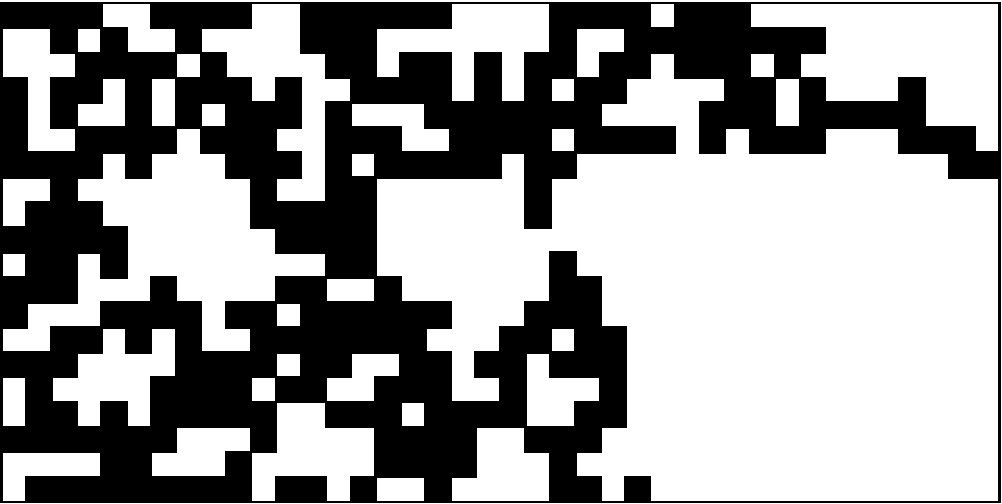
\includegraphics[width=12.0cm]{figure_1.pdf}
                       \caption{$20\times 40$の格子上で得られた侵略型パーコレーションのクラスター}
                       \label{fig:14-7-f1}
                   \end{center}
               \end{figure}
               
            \end{enumerate}    
        
        \item 侵略者が初めて右の端に達したとき,$L\times 2L$の格子の中央の$L\times L$の領域で,侵略者によって占有された格子点の数$M(L)$を少なくとも20回の試行について平均せよ.$M(L) \sim L^{D}$を仮定し,$\ln M$の$\ln L$に対するプロットから$D$の値を求めよ.得られた$D$の値と通常のパーコレーションのフラクタル次元とを比較せよ.(発表されているWilkinsonとWillemsenによって計算された$M(L)$の値は,$L$の20から100の範囲について各2000回の試行結果から得られている.)
        
            \begin{enumerate}
                \item $L$の20から100の範囲の10個の$L$について,それぞれ100回の試行の平均からフラクタル次元$D$を計算した.横軸を$\ln L$,縦軸を$\ln M(L)$としてプロットしたものを図\ref{fig:14-7-f2}に示す.この傾きは$D\simeq 1.92$と求められた.これは通常のパーコレーションモデルによって得られたクラスターのフラクタル次元$D\simeq 1.89$とも近い値となっている.また,侵略型パーコレーションクラスターの,大規模なシミュレーションによって得られたフラクタル次元の値も$D\simeq 1.89$であり,全く違う機構で生成されたクラスターのフラクタル次元が一致するということは大変興味深い.
                
                \begin{figure}[H]
                    \begin{center}
                        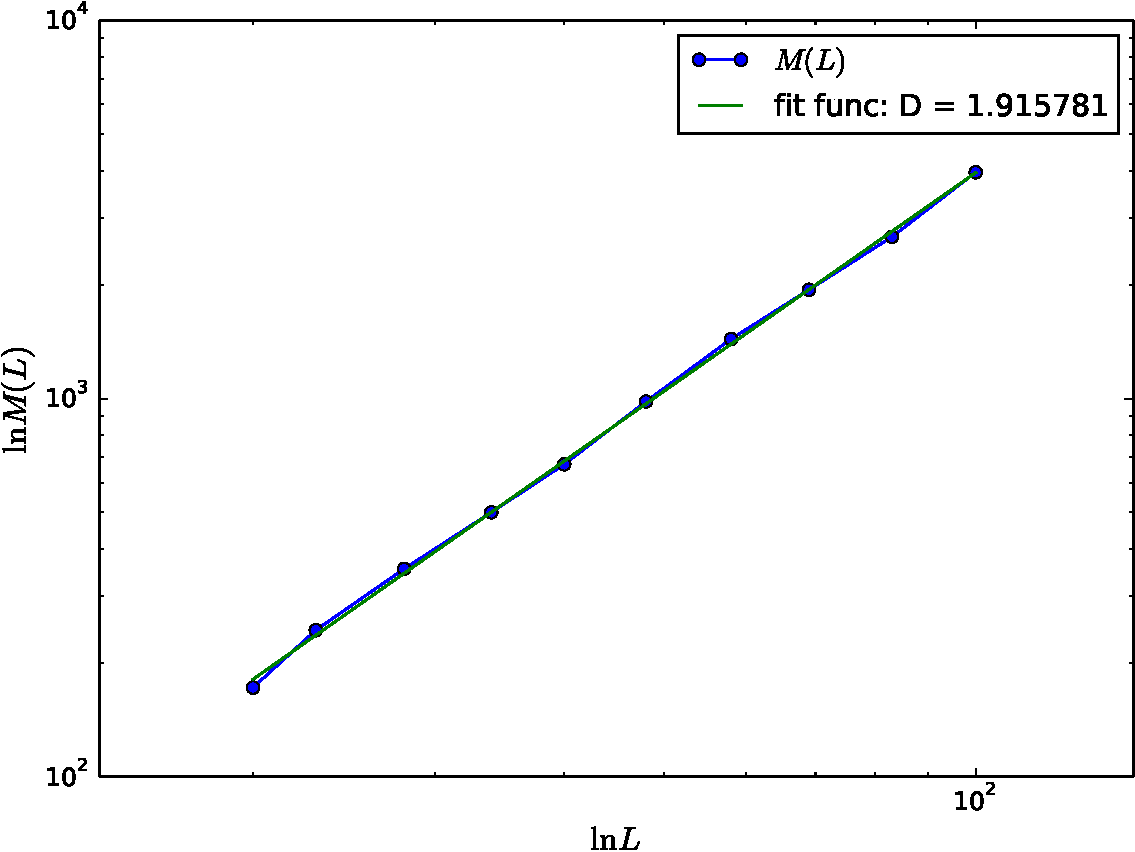
\includegraphics[width=12.0cm]{figure_2.pdf}
                        \caption{$\ln M$の$\ln L$に対するプロット}
                        \label{fig:14-7-f2}
                    \end{center}
                \end{figure}
                
            \end{enumerate} 
        
    \end{enumerate}

\section{まとめ}

    侵略型パーコレーションモデルによるクラスターを作成し,そのフラクタル次元が通常のパーコレーションクラスターのフラクタル次元と等しくなることを見た.また,冒頭で侵略型パーコレーションモデルの誕生の経緯として,油を含んだ多孔性の媒体に水を押しこんで油を取り出すことを考えていたが,クラスターのフラクタル次元が$D<d$であることから,効率よく油を採取することはできないということもわかる.

\nocite{textbook}
\nocite{fractal1}
\bibliography{/home/shotaro/Workspace/computing_simulation/reference}


\end{document}
